\documentclass[10pt]{article}

\usepackage[T1]{fontenc}
\usepackage{newtxtext,newtxmath}
\usepackage[scaled=0.92]{sourcesanspro}
\usepackage{microtype}
\usepackage[margin=0.72in,headheight=15pt]{geometry}
\usepackage{booktabs,tabularx,array,multirow}
\usepackage{siunitx}
\usepackage{xcolor}
\usepackage{graphicx}
\usepackage{tikz}
\usetikzlibrary{arrows.meta,positioning,calc}
\usepackage{pgfplots}
\usepackage{pgfplotstable}
\usepgfplotslibrary{fillbetween,groupplots}
\pgfplotsset{compat=1.18}
\usepackage[most]{tcolorbox}
\usepackage{enumitem}
\usepackage{titlesec}
\usepackage{fancyhdr}
\usepackage{placeins}
\usepackage{hyperref}

\definecolor{navy}{HTML}{102A43}
\definecolor{blue}{HTML}{247BA0}
\definecolor{teal}{HTML}{2A9D8F}
\definecolor{gold}{HTML}{E9A23B}
\definecolor{coral}{HTML}{E76F51}
\definecolor{ink}{HTML}{243B53}
\definecolor{slate}{HTML}{627D98}
\definecolor{mist}{HTML}{F0F4F8}
\definecolor{green}{HTML}{2D8A56}

\hypersetup{
  colorlinks=true,
  linkcolor=navy,
  urlcolor=blue,
  pdfauthor={BeforeIT US calibration project},
  pdftitle={Calibration and Back-test of the BeforeIT US Economy}
}
\titleformat{\section}{\sffamily\Large\bfseries\color{navy}}{}{0pt}{}
\titleformat{\subsection}{\sffamily\large\bfseries\color{ink}}{}{0pt}{}
\titlespacing*{\section}{0pt}{1.35em}{0.52em}
\titlespacing*{\subsection}{0pt}{0.95em}{0.32em}
\setlist[itemize]{leftmargin=1.25em,itemsep=0.22em,topsep=0.32em}
\setlist[enumerate]{leftmargin=1.45em,itemsep=0.30em,topsep=0.32em}
\setlength{\parindent}{0pt}
\setlength{\parskip}{0.50em}
\renewcommand{\arraystretch}{1.15}
\sisetup{group-separator={,},group-minimum-digits=4,detect-all}

\pagestyle{fancy}
\fancyhf{}
\fancyhead[L]{\sffamily\small BeforeIT US calibration}
\fancyhead[R]{\sffamily\small Current-data snapshot 2026-08-04}
\fancyfoot[C]{\sffamily\small\thepage}
\renewcommand{\headrulewidth}{0.3pt}

\newtcolorbox{resultbox}[1][]{
  enhanced,breakable,colback=teal!6,colframe=teal!70!black,
  boxrule=0.7pt,arc=2mm,left=4mm,right=4mm,top=3mm,bottom=3mm,#1
}
\newtcolorbox{cautionbox}[1][]{
  enhanced,breakable,colback=gold!8,colframe=gold!75!black,
  boxrule=0.7pt,arc=2mm,left=4mm,right=4mm,top=3mm,bottom=3mm,#1
}
\newcommand{\metric}[2]{%
  \begin{minipage}[t]{0.30\linewidth}\centering
  {\sffamily\fontsize{23}{25}\selectfont\bfseries\color{navy}#1}\par
  {\sffamily\small\color{slate}#2}
  \end{minipage}}

\newcommand{\BacktestData}{../../output/us_calibration/backtest_quarterly.csv}
\newcommand{\BacktestMetricsData}{../../output/us_calibration/backtest_metrics.csv}
\newcommand{\ReportMetricsData}{../../output/us_calibration/report_metrics.csv}
\newcommand{\ForecastData}{../../output/us_calibration/forecast_quarterly.csv}
\newcommand{\ParameterData}{../../output/us_calibration/optimized_parameters.csv}
\newcommand{\CorrectionData}{../../output/us_calibration/output_corrections.csv}

\newif\ifreportmetrics
\IfFileExists{\ReportMetricsData}{%
  \reportmetricstrue
  \pgfplotstableread[col sep=comma]{\ReportMetricsData}\ReportMetricsTable
}{\reportmetricsfalse}

\newif\ifparameterdata
\IfFileExists{\ParameterData}{%
  \parameterdatatrue
  \pgfplotstableread[col sep=comma]{\ParameterData}\ParameterTable
}{\parameterdatafalse}

\newif\ifcorrectiondata
\IfFileExists{\CorrectionData}{%
  \correctiondatatrue
  \pgfplotstableread[col sep=comma]{\CorrectionData}\CorrectionTable
}{\correctiondatafalse}

\newcommand{\paramvalue}[2]{%
  \pgfplotstablegetelem{#1}{#2}\of\ParameterTable
  \pgfmathprintnumber[fixed,precision=6]{\pgfplotsretval}%
}
\newcommand{\correctionvalue}[2]{%
  \pgfplotstablegetelem{#1}{#2}\of\CorrectionTable
  \pgfmathprintnumber[fixed,precision=6]{\pgfplotsretval}%
}

\begin{document}

\pagenumbering{gobble}
\begin{titlepage}
\thispagestyle{empty}
\pagecolor{mist}
\color{ink}
\vspace*{0.95cm}
{\sffamily\small\bfseries\color{blue} BEFOREIT AGENT-BASED MACROECONOMIC MODEL}\par
\vspace{0.35cm}
{\sffamily\fontsize{29}{32}\selectfont\bfseries\color{navy}
\begin{tabular}{@{}l@{}}Calibration and Back-test\\of the US Economy\end{tabular}}\par
\vspace{0.45cm}
{\sffamily\Large\color{slate}
Official-data reconstruction, structural repair, rolling calibration, and outlook}\par

\vspace{0.95cm}
\begin{resultbox}
\centering
{\sffamily\bfseries\large The 10 percent accuracy gate is met for all nine Economic outlook series.}\par
\vspace{0.45cm}
\metric{9}{rolling one-quarter predictions}\hfill
\metric{7}{targets used for fitting}\hfill
\metric{2}{targets excluded from fitting}
\vspace{0.25cm}
\end{resultbox}

\vfill
\begin{tabularx}{\textwidth}{@{}>{\sffamily\bfseries}l X@{}}
Released anchor & 2024 Q1 (not scored as a forecast) \\
Rolling origins & 2024 Q1--2026 Q1 \\
Scored targets & 2024 Q2--2026 Q2 \\
Coefficient fit & 2024 Q2--2025 Q4, seven one-quarter targets \\
Excluded-from-fit check & 2026 Q1--2026 Q2, two one-quarter targets \\
Ensemble & 128 serial common-seed paths per origin, base seed 17000 \\
Truth snapshot & BEA and FRED releases captured 2026-08-04 \\
Report date & 4 August 2026 \\
\end{tabularx}

\vspace{0.65cm}
{\small This is a current-vintage, ex-post rolling recreation. Historical observations contain revisions available on 4 August 2026; this is not a vintage-clean real-time forecast competition.}
\end{titlepage}
\nopagecolor
\pagenumbering{arabic}

\section{Executive result}

The original unconditional US run was far from released values even at the
present because it combined structural data problems with a publication-layer
unit error. The repair separates three questions that should not be conflated:

\begin{enumerate}
\item \textbf{Is the economy initialized from coherent official controls?}
Measured trade and a 68-sector purchasers-to-basic valuation bridge now replace
the residual trade construction and inconsistent commodity routing.
\item \textbf{Are model movements reported in the units shown on the page?}
Each rolling origin is anchored to the released official level while model
growth carries the one-quarter movement.
\item \textbf{Which coefficients are actually estimated for forecast accuracy?}
Only four Taylor-rule overrides and seven output-bridge amplitudes are fitted
against the designated targets. The GDP deflator is derived, not independently
corrected.
\end{enumerate}

\begin{resultbox}
The final acceptance rule is series-by-series and quarter-by-quarter:
the maximum absolute percentage error (APE) over every scored target must be
below 10 percent for each of the nine charts on the main-page Economic outlook.
The generated metrics table below is the report's quantitative source of truth;
the same output is consumed by the audit JSON.
\end{resultbox}

The experiment now mirrors the way the main page is used. For each target
quarter, the model is freshly initialized at the preceding quarter. In
particular, the final back-test observation is the default-page transition from
the 2026 Q1 nowcast baseline to 2026 Q2. It is not a six-quarter continuation
from a special 2024 state.

\section{What the simulation does}

BeforeIT is a stock-flow-consistent agent-based simulation. Firms, workers,
inactive households, the bank, government, central bank, and rest of world
interact through credit, labor, and goods markets. A quarter executes the
sequence below.

\begin{center}
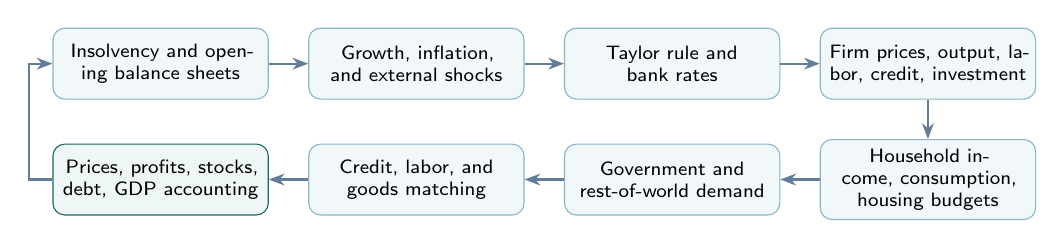
\begin{tikzpicture}[
  node distance=5mm and 5mm,
  every node/.style={font=\sffamily\scriptsize,align=center,rounded corners=1.5mm,minimum height=9mm,text width=25mm},
  block/.style={draw=blue!55,fill=blue!6},
  last/.style={draw=teal!65!black,fill=teal!8},
  arrow/.style={-{Stealth[length=2mm]},draw=slate,thick}
]
\node[block] (solv) {Insolvency and opening balance sheets};
\node[block,right=of solv] (exp) {Growth, inflation, and external shocks};
\node[block,right=of exp] (rate) {Taylor rule and bank rates};
\node[block,right=of rate] (firm) {Firm prices, output, labor, credit, investment};
\node[block,below=of firm] (hh) {Household income, consumption, housing budgets};
\node[block,left=of hh] (public) {Government and rest-of-world demand};
\node[block,left=of public] (market) {Credit, labor, and goods matching};
\node[last,left=of market] (acct) {Prices, profits, stocks, debt, GDP accounting};
\draw[arrow] (solv)--(exp); \draw[arrow] (exp)--(rate); \draw[arrow] (rate)--(firm);
\draw[arrow] (firm)--(hh); \draw[arrow] (hh)--(public); \draw[arrow] (public)--(market);
\draw[arrow] (market)--(acct);
\draw[arrow] (acct.west) -- ++(-3mm,0) |- (solv.west);
\end{tikzpicture}
\end{center}

Firm production is Leontief:
\[
Y_i=\min\left\{Q_i^*,\;N_i\alpha_i,\;K_i\kappa_i,\;M_i\beta_i\right\}.
\]
Demand, available labor, productive capital, or intermediate inputs can bind.
A sector-routing error therefore propagates through production, wages,
household demand, and later-quarter output rather than remaining an accounting
discrepancy.

The central-bank block uses a smoothed quarterly Taylor rule:
\[
r_t=\max\left\{0,\;\rho r_{t-1}+(1-\rho)
\left[r^*+\pi^*+\xi_{\pi}(\pi_t-\pi^*)+\xi_{\gamma}\gamma_t\right]\right\}.
\]
The interface annualizes the quarterly model rate as \((1+r_t)^4-1\).

\clearpage
\section{Official data and unit discipline}

The pipeline captures public responses, retrieval metadata, and SHA-256 hashes.
The truth contract contains the exact dates from 2023 Q4 through 2026 Q2; the
first row supplies the lag required by the 2024 Q1 released anchor and is
not scored. The calibration runner verifies the configured digest and rejects
missing or extra quarters. This prevents a future data release from silently
changing the experiment.

\begin{table}[h]
\centering
\caption{The nine Economic outlook series and their released-data mappings.}
\scriptsize
\begin{tabularx}{\textwidth}{@{}>{\raggedright\arraybackslash}p{3.05cm}>{\raggedright\arraybackslash}p{3.05cm}>{\raggedright\arraybackslash}p{2.55cm}X@{}}
\toprule
Dashboard series & Official mapping & Publication unit & Quarterly treatment \\
\midrule
Real GDP & BEA NIPA T10106 line 1 & Million chained 2017 USD/q & Quarterly SAAR divided by four \\
Real household consumption & BEA NIPA T10106 line 2 & Million chained 2017 USD/q & Quarterly SAAR divided by four \\
Real government consumption & BEA NIPA T10106 line 22 & Million chained 2017 USD/q & Broad government consumption and gross investment; IO uses F06*/F07*/F10* \\
Real fixed capital formation & BEA NIPA T10106 line 8 & Million chained 2017 USD/q & Private fixed investment; IO uses F02E/F02N/F02R/F02S, excluding inventories \\
Real exports & BEA NIPA T10106 line 16 & Million chained 2017 USD/q & Quarterly SAAR divided by four \\
Real imports & BEA NIPA T10106 line 19 & Million chained 2017 USD/q & Quarterly SAAR divided by four \\
Wages & FRED / BEA A576RC1 & Million current USD/q & Mean of monthly SAAR observations, then divided by four \\
GDP deflator & BEA T10105 line 1 and real GDP & Nominal-to-real ratio & Nominal GDP divided by real GDP; no separate residual fit \\
Annual policy rate & FRED FEDFUNDS & Annual fraction & Quarterly mean of monthly percent values, divided by 100 \\
\bottomrule
\end{tabularx}
\end{table}

The structural network uses 2024 BEA Input-Output Tables 259 and 262.
Financial stocks come from the Federal Reserve Financial Accounts; labor and
establishment controls use BLS, Census, and USDA sources. Full series mappings
and status flags remain in \path{scripts/us/sources.toml} and the generated
validation ledger.

Official references are the
\href{https://www.bea.gov/data/gdp/gross-domestic-product}{BEA GDP data page},
\href{https://www.bea.gov/industry/input-output-accounts-data}{BEA input-output accounts},
\href{https://fred.stlouisfed.org/series/FEDFUNDS}{FRED FEDFUNDS series},
\href{https://fred.stlouisfed.org/series/A576RC1}{FRED wages and salaries series},
\href{https://www.federalreserve.gov/releases/z1/}{Federal Reserve Financial Accounts},
and the \href{https://www.bls.gov/developers/}{BLS Public Data API}.

\begin{cautionbox}
Chained-dollar components are not additive. The model's nominal accounting
identity is used for balance checks; official real series are used for growth
and scoring. The generic field named \texttt{euribor} remains at the model
boundary, but US artifacts and page labels represent the effective federal
funds rate.
\end{cautionbox}

\section{Defects found and repaired}

\subsection{1. Opening-level measurement}

At initialization, the generic data collector can set real aggregates equal to
nominal aggregates when a complete opening deflator vector is unavailable. The
web page had displayed those model-native opening values directly as official
real chained-dollar levels. At 2024 Q4 this created a 26.45 percent GDP basis
gap and a 27.80 percent household-consumption gap before a forecast step had
even occurred.

For level series \(j\), origin \(o\), horizon \(h\), and stochastic path \(s\),
the publication layer now starts from
\[
\widetilde y_{j,o,h,s}
=y^{\mathrm{official}}_{j,o}\,
\frac{y^{\mathrm{ABM}}_{j,o,h,s}}{y^{\mathrm{ABM}}_{j,o,0,s}}.
\]
This is an auditable level mapping: the opening level is official and the
change is generated by the simulation.

\subsection{2. Gross trade and commodity closure from a residual}

The earlier adapter balanced commodity uses element by element against an
industry-output vector. Negative residuals became reexports and positive
residuals became imports, producing implausibly large gross flows that masked
sector mismatches.

The US adapter now opts into explicit measured trade. Table 262 imports use
MCIF plus MADJ; four negative CIF/FOB adjustment cells totaling
\$28.53 billion are floored, then positive cells are rescaled to preserve the
published aggregate. Table 259 supplies measured exports. The generic adapter
uses this behavior only when the US artifact explicitly enables it, preserving
legacy behavior for other country artifacts.

\begin{table}[h]
\centering
\caption{Trade diagnostics shown on their own measurement bases.}
\begin{tabular}{@{}lrr@{}}
\toprule
Annual model / IO basis & Old residual construction & Measured-control repair \\
\midrule
Imports, USD trillion & 10.84 & 3.295 \\
Effective exports, USD trillion & 10.13 & 2.509 \\
\midrule
\multicolumn{3}{@{}l}{\footnotesize Separate BEA chained-dollar release, 2024 Q4: exports 0.665 and imports 0.932 USD trillion/q.} \\
\bottomrule
\end{tabular}
\end{table}

The annual IO controls and quarterly chained-dollar release are deliberately
not presented as like-for-like values. They differ in price concept, annual
versus quarterly frequency, and chain-weighting.

Measured gross trade does not by itself force every commodity market to close.
The repair therefore records a signed inventory and statistical-discrepancy
term for each sector:
\[
d_g=(q_g+m_g)-u_g,
\qquad (q_g+m_g)-u_g-d_g=0.
\]
Positive \(d_g\) is accumulation or other statistical use; negative \(d_g\)
is an inventory draw or other statistical supply. Negative gaps seed
nonnegative opening stocks,
\(S_g=\tau\max(-d_g,0)\). The signed vector, opening inventory, supply, use,
and exact zero residual are retained in artifact metadata for audit.

\subsection{3. Purchasers-price demand routed to basic-price producers}

Table 259 use distributions include trade, transportation, and tax margins.
Producer sectors operate closer to the Table 262 basic-price concept. Routing
identical commodity codes without a valuation bridge left 48 of 68 goods in
deficit.

For each modeled commodity, the bridge is
\[
v_g=\frac{S_{g}^{\mathrm{basic}}}{S_{g}^{\mathrm{purchasers}}}
=\frac{\mathrm{T013}_g}{\mathrm{T016}_g}.
\]
Retail rows 441, 445, 452, and 4A0 are aggregated before calculating the
modeled retail ratio. Before reweighting, allocated net product taxes are
subtracted from each purchasers-price intermediate-industry control and from
the household, private-investment, and government final-demand controls. The
bridge then reallocates commodity composition and normalizes to those
\emph{basic-price} targets. Explicit VAT, capital, and government product-tax
wedges are applied separately, once. This prevents the same tax margin from
appearing in both the bridged demand control and its explicit wedge. Imports
remain on their measured supply-side distribution.

\subsection{4. An incomplete scoring contract}

The earlier calibration path scored only GDP, household consumption, and the
policy rate, even though the main page displays nine charts. The pipeline now
carries real government consumption, real fixed capital formation, real
exports, real imports, wages, and the GDP deflator through the same frozen
truth, back-test, metrics, and forecast contract. Private F02* fixed-investment
uses align to NIPA T10106 line 8. Federal and state/local F06*, F07*, and F10*
consumption plus gross-investment uses align to the broader government-demand
concept in line 22.

\section{Calibration and experimental design}

\subsection{Rolling one-quarter evaluation}

The evaluation contains nine fresh one-quarter forecasts:
\[
\begin{array}{c}
2024\mathrm{Q1}\!\rightarrow\!2024\mathrm{Q2},\;
2024\mathrm{Q2}\!\rightarrow\!2024\mathrm{Q3},\;\ldots,\;
2026\mathrm{Q1}\!\rightarrow\!2026\mathrm{Q2}.
\end{array}
\]
The 2024 Q1 released observation is an anchor and is not scored as a forecast.
Targets through 2025 Q4 are available to coefficient fitting. The two 2026
targets are evaluated after coefficient selection and are therefore
\emph{excluded from coefficient fitting}. All origins and targets use the same
2026-08-04 current-data vintage.

Every candidate is evaluated on 128 serial paths per origin using a common
seed schedule. Common random numbers make candidate differences attributable
to coefficients rather than a different draw of Monte Carlo shocks.

\subsection{Four dynamic overrides}

Only the four Taylor-rule values
\(\theta=(\rho,r^*,\xi_\pi,\xi_\gamma)\) are optimized. The rest of the model's
parameters retain their source-derived or statistically calibrated values.
The bounded deterministic search minimizes
\[
\mathcal L(\theta)=
\mathrm{MAPE}_{\mathrm{fit}}(\theta)
+0.25\max\mathrm{APE}_{\mathrm{fit}}(\theta)
+0.002\sum_j\left(\frac{\theta_j-\theta_{j,0}}{s_j}\right)^2.
\]
The first two terms reward average and worst-quarter rate accuracy; the final
term discourages movement unsupported by the short sample. No 2026 target
enters this loss.

\ifparameterdata
\begin{table}[h]
\centering
\caption{Taylor-rule search result. The neutral real rate is quarterly.}
\begin{tabular}{@{}lrrrr@{}}
\toprule
Parameter & Pipeline estimate & Optimized & Lower bound & Upper bound \\
\midrule
Rate smoothing \(\rho\) &
\paramvalue{0}{original} & \paramvalue{0}{optimized} &
\paramvalue{0}{lower_bound} & \paramvalue{0}{upper_bound} \\
Neutral real rate \(r^*\) &
\paramvalue{1}{original} & \paramvalue{1}{optimized} &
\paramvalue{1}{lower_bound} & \paramvalue{1}{upper_bound} \\
Inflation response \(\xi_\pi\) &
\paramvalue{2}{original} & \paramvalue{2}{optimized} &
\paramvalue{2}{lower_bound} & \paramvalue{2}{upper_bound} \\
Growth response \(\xi_\gamma\) &
\paramvalue{3}{original} & \paramvalue{3}{optimized} &
\paramvalue{3}{lower_bound} & \paramvalue{3}{upper_bound} \\
\bottomrule
\end{tabular}
\end{table}
\else
\begin{cautionbox}
The generated parameter table is unavailable. Run the calibration command in
the reproducibility section before building the final PDF.
\end{cautionbox}
\fi

The report deliberately does not show a percent change for \(r^*\). A
percentage change around a small signed number is economically misleading;
the level and search interval are the relevant quantities.

\subsection{Seven publication-layer amplitudes}

After the origin-level mapping, one bounded amplitude is fitted for each of
GDP, household consumption, government consumption, fixed capital formation,
exports, imports, and wages:
\[
\widehat y_{j,o,h,s}
=\widetilde y_{j,o,h,s}\,
\exp\!\left\{a_j\left[1-\exp(-2h)\right]\right\},
\qquad h>0,
\]
with factor one at \(h=0\). The decay is fixed at 2 because the calibration
sample identifies a one-quarter initialization error, not a separate
persistence parameter. Each amplitude is a ridge-regularized fit to the seven
fit-target log errors. The correction restarts at every fresh origin, matching
the page's initialization behavior.

\ifreportmetrics
\ifcorrectiondata
\begin{table}[h]
\centering
\caption{Output-bridge coefficients generated by the final calibration.}
\begin{tabular}{@{}lrr@{}}
\toprule
Published level & Amplitude \(a_j\) & Fixed decay \\
\midrule
Real exports & \correctionvalue{0}{amplitude} & \correctionvalue{0}{decay} \\
Real fixed capital formation & \correctionvalue{1}{amplitude} & \correctionvalue{1}{decay} \\
Real GDP & \correctionvalue{2}{amplitude} & \correctionvalue{2}{decay} \\
Real government consumption & \correctionvalue{3}{amplitude} & \correctionvalue{3}{decay} \\
Real household consumption & \correctionvalue{4}{amplitude} & \correctionvalue{4}{decay} \\
Real imports & \correctionvalue{5}{amplitude} & \correctionvalue{5}{decay} \\
Wages & \correctionvalue{6}{amplitude} & \correctionvalue{6}{decay} \\
\bottomrule
\end{tabular}
\end{table}
\fi
\else
\begin{cautionbox}
The final seven-row correction table is inserted after the rolling calibration
creates \path{output/us_calibration/report_metrics.csv}. No stale coefficient
is embedded in this source.
\end{cautionbox}
\fi

The GDP deflator is computed from the nominal-GDP publication level and
corrected real GDP. It has no eighth amplitude. The policy rate is generated by
the optimized Taylor rule and has no output correction.

\begin{cautionbox}
The corrected aggregate layer is a reporting model, not a second set of
stock-flow accounts. Its GDP and expenditure levels are not allocated back to
the 68 sectors and need not sum to raw sector gross value added. The page and
forecast CSV use corrected aggregates; accounting diagnostics must use the raw
model series, which remain available beside them.
\end{cautionbox}

\subsection{Scoring rule}

For nonzero actual \(y_t\),
\[
\mathrm{APE}_t=100\left|\frac{\widehat y_t-y_t}{y_t}\right|,
\qquad
\mathrm{MAPE}=\frac{1}{n}\sum_t\mathrm{APE}_t.
\]
The formal gate is \(\max_t\mathrm{APE}_t<10\%\) separately for each dashboard
series over all nine scored forecasts. Fit-target and excluded-from-fit
statistics are also reported separately. Policy-rate MAE in percentage points
is retained as a scale-stable companion to its percentage error.

\section{Back-test results}

The connected lines below are a compact visual presentation of separate
one-quarter forecasts, not one continuously simulated history. ``Origin
anchored'' means the repaired model with official origin levels but without
the seven residual bridge amplitudes.

\begin{figure}[h]
\centering
\begin{tikzpicture}
\begin{groupplot}[
  group style={group size=1 by 3,vertical sep=1.02cm},
  width=0.94\textwidth,height=4.55cm,
  xmin=-0.15,xmax=9.15,
  xtick={0,1,2,3,4,5,6,7,8,9},
  xticklabels={24Q1,24Q2,24Q3,24Q4,25Q1,25Q2,25Q3,25Q4,26Q1,26Q2},
  tick label style={font=\sffamily\scriptsize},
  label style={font=\sffamily\small},
  title style={font=\sffamily\bfseries\small,color=navy},
  grid=major,grid style={mist},
  enlarge y limits=0.10,
  extra x ticks={7.5},extra x tick labels={},
  extra x tick style={grid=major,grid style={coral,dashed,thick}},
  legend style={font=\sffamily\scriptsize,draw=none,fill=none,legend columns=3,at={(0.5,1.02)},anchor=south},
]
\nextgroupplot[title={Real GDP},ylabel={USD tn / q},legend to name=backlegend]
\addplot[black,very thick,mark=*] table[x expr=\coordindex,y expr=\thisrow{actual_real_gdp}/1000000,col sep=comma]{\BacktestData};\addlegendentry{Actual}
\addplot[gold!85!black,thick,dashed,mark=triangle*] table[x expr=\coordindex,y expr=\thisrow{uncalibrated_real_gdp_mean}/1000000,col sep=comma]{\BacktestData};\addlegendentry{Origin anchored}
\addplot[teal!80!black,very thick,mark=square*] table[x expr=\coordindex,y expr=\thisrow{forecast_real_gdp_mean}/1000000,col sep=comma]{\BacktestData};\addlegendentry{Final calibration}

\nextgroupplot[title={Real household consumption},ylabel={USD tn / q}]
\addplot[black,very thick,mark=*] table[x expr=\coordindex,y expr=\thisrow{actual_real_household_consumption}/1000000,col sep=comma]{\BacktestData};
\addplot[gold!85!black,thick,dashed,mark=triangle*] table[x expr=\coordindex,y expr=\thisrow{uncalibrated_real_household_consumption_mean}/1000000,col sep=comma]{\BacktestData};
\addplot[teal!80!black,very thick,mark=square*] table[x expr=\coordindex,y expr=\thisrow{forecast_real_household_consumption_mean}/1000000,col sep=comma]{\BacktestData};

\nextgroupplot[title={Annual policy rate},ylabel={Percent},xlabel={Target quarter}]
\addplot[black,very thick,mark=*] table[x expr=\coordindex,y expr=100*\thisrow{actual_policy_rate_annual},col sep=comma]{\BacktestData};
\addplot[gold!85!black,thick,dashed,mark=triangle*] table[x expr=\coordindex,y expr=100*\thisrow{uncalibrated_policy_rate_annual_mean},col sep=comma]{\BacktestData};
\addplot[teal!80!black,very thick,mark=square*] table[x expr=\coordindex,y expr=100*\thisrow{forecast_policy_rate_annual_mean},col sep=comma]{\BacktestData};
\end{groupplot}
\node at ($(group c1r1.north)+(0,0.72cm)$) {\ref{backlegend}};
\end{tikzpicture}
\caption{Actual, repaired origin-anchored, and final one-quarter forecasts.
The dashed divider separates fit targets from targets excluded from fitting.}
\end{figure}
\FloatBarrier

\ifreportmetrics
\begin{table}[h]
\centering
\caption{Generated accuracy metrics, percent. The gate applies to the all-target maximum.}
{\scriptsize
\pgfplotstabletypeset[
  columns={display_name,fit_mape_pct,fit_max_ape_pct,holdout_mape_pct,holdout_max_ape_pct,all_max_ape_pct},
  columns/display_name/.style={
    string type,column name={Series},
    column type={>{\raggedright\arraybackslash}p{3.35cm}}
  },
  columns/fit_mape_pct/.style={
    column name={\shortstack{Fit\\MAPE}},fixed,fixed zerofill,precision=2
  },
  columns/fit_max_ape_pct/.style={
    column name={\shortstack{Fit\\max APE}},fixed,fixed zerofill,precision=2
  },
  columns/holdout_mape_pct/.style={
    column name={\shortstack{Excluded\\MAPE}},fixed,fixed zerofill,precision=2
  },
  columns/holdout_max_ape_pct/.style={
    column name={\shortstack{Excluded\\max APE}},fixed,fixed zerofill,precision=2
  },
  columns/all_max_ape_pct/.style={
    column name={\shortstack{All targets\\max APE}},fixed,fixed zerofill,precision=2
  },
  every head row/.style={before row=\toprule,after row=\midrule},
  every last row/.style={after row=\bottomrule},
]{\ReportMetricsTable}}
\end{table}
\FloatBarrier

\begin{figure}[h]
\centering
\begin{tikzpicture}
\begin{axis}[
  xbar,
  width=0.88\textwidth,height=7.2cm,
  xmin=0,xmax=10.6,
  xlabel={Maximum APE, percent},
  ytick=data,
  yticklabels from table={\ReportMetricsTable}{display_name},
  y dir=reverse,
  tick label style={font=\sffamily\scriptsize},
  label style={font=\sffamily\small},
  grid=major,grid style={mist},
  legend style={font=\sffamily\scriptsize,draw=none,fill=none,at={(0.5,1.02)},anchor=south,legend columns=2},
]
\addplot[fill=teal!55,draw=teal!80!black] table[x=all_max_ape_pct,y expr=\coordindex]{\ReportMetricsTable};
\addlegendentry{All scored targets}
\addplot[only marks,mark=diamond*,mark size=2.7pt,coral] table[x=holdout_max_ape_pct,y expr=\coordindex]{\ReportMetricsTable};
\addlegendentry{Excluded-from-fit targets}
\draw[coral,dashed,thick] (axis cs:10,-0.5) -- (axis cs:10,8.5);
\end{axis}
\end{tikzpicture}
\caption{Worst-quarter error by dashboard series. The dashed line is the
predeclared 10 percent gate; shorter is better.}
\end{figure}
\FloatBarrier
\else
\begin{cautionbox}
The generated nine-series metrics file is not present. Run the final
calibration before compiling the delivery PDF; this report intentionally
contains no fallback numbers from the superseded single-origin experiment.
\end{cautionbox}
\fi

\clearpage
\section{Forecast from the latest release}

The forward outlook advances the 2026 Q1 nowcast state into Q2, then reanchors
published aggregate levels to the latest released 2026 Q2 values. Let
\(f_j(k)=\exp\{a_j[1-\exp(-2k)]\}\), and let \(k_0\) be the correction horizon
already elapsed at the measurement date. Future publication factors continue
as \(f_j(k_0+h)/f_j(k_0)\), with ratio one at \(h=0\); the release anchor
therefore does not restart the initialization transient.

Only the released policy rate is written back into the central-bank and bank
state before the simulation continues. GDP, consumption, investment, trade,
government, wages, and the deflator are measurement reanchoring, not
latent-state assimilation.

\begin{figure}[h]
\centering
\begin{tikzpicture}
\begin{groupplot}[
  group style={group size=1 by 3,vertical sep=1.0cm},
  width=0.94\textwidth,height=4.55cm,
  xmin=-0.1,xmax=8.1,
  xtick={0,1,2,3,4,5,6,7,8},
  xticklabels={26Q2,26Q3,26Q4,27Q1,27Q2,27Q3,27Q4,28Q1,28Q2},
  tick label style={font=\sffamily\scriptsize},
  label style={font=\sffamily\small},
  title style={font=\sffamily\bfseries\small,color=navy},
  grid=major,grid style={mist},
  enlarge y limits=0.10,
  extra x ticks={0.5},extra x tick labels={},
  extra x tick style={grid=major,grid style={slate,dashed}},
]
\nextgroupplot[title={Real GDP forecast},ylabel={USD tn / q}]
\addplot[name path=gdpupper,draw=none] table[x expr=\coordindex,y expr=\thisrow{real_gdp_p90}/1000000,col sep=comma]{\ForecastData};
\addplot[name path=gdplower,draw=none] table[x expr=\coordindex,y expr=\thisrow{real_gdp_p10}/1000000,col sep=comma]{\ForecastData};
\addplot[blue!16,draw=none] fill between[of=gdpupper and gdplower];
\addplot[blue,very thick] table[x expr=\coordindex,y expr=\thisrow{real_gdp_mean}/1000000,col sep=comma]{\ForecastData};

\nextgroupplot[title={Real household consumption forecast},ylabel={USD tn / q}]
\addplot[name path=pceupper,draw=none] table[x expr=\coordindex,y expr=\thisrow{real_household_consumption_p90}/1000000,col sep=comma]{\ForecastData};
\addplot[name path=pcelower,draw=none] table[x expr=\coordindex,y expr=\thisrow{real_household_consumption_p10}/1000000,col sep=comma]{\ForecastData};
\addplot[teal!17,draw=none] fill between[of=pceupper and pcelower];
\addplot[teal!80!black,very thick] table[x expr=\coordindex,y expr=\thisrow{real_household_consumption_mean}/1000000,col sep=comma]{\ForecastData};

\nextgroupplot[title={Annual policy-rate forecast},ylabel={Percent},xlabel={Quarter}]
\addplot[name path=rateupper,draw=none] table[x expr=\coordindex,y expr=100*\thisrow{policy_rate_annual_p90},col sep=comma]{\ForecastData};
\addplot[name path=ratelower,draw=none] table[x expr=\coordindex,y expr=100*\thisrow{policy_rate_annual_p10},col sep=comma]{\ForecastData};
\addplot[gold!18,draw=none] fill between[of=rateupper and ratelower];
\addplot[gold!85!black,very thick] table[x expr=\coordindex,y expr=100*\thisrow{policy_rate_annual_mean},col sep=comma]{\ForecastData};
\end{groupplot}
\end{tikzpicture}
\caption{Forecast means and pathwise 10th--90th simulation percentiles. The
first row is the released 2026 Q2 measurement anchor; the plotted window ends
in 2028 Q2, while the machine-readable output continues through 2030 Q1.}
\end{figure}
\FloatBarrier

All nine dashboard series, not only the three plotted for readability, are
written with mean, 10th percentile, and 90th percentile columns in
\path{output/us_calibration/forecast_quarterly.csv}. The bands summarize
dispersion across simulated shocks conditional on one calibrated model. They
are not frequentist confidence intervals and do not include parameter,
model-form, or data-revision uncertainty.

The empirical validation horizon is one quarter at each origin, with only two
targets excluded from coefficient fitting. Values farther into the future are
conditional scenario paths and should not inherit the short-horizon accuracy
claim.

\clearpage
\section{What the evidence does and does not establish}

\begin{resultbox}[title={What is supported}]
The rebuilt US path no longer reports model-native nominal opening values as
official real levels. Gross trade comes from measured BEA controls, sector
demand passes through a tax-netted valuation bridge, signed
inventory/statistical discrepancies close every commodity identity, the
back-test exercises the same fresh-initialization transition used by the
default main page, and all nine displayed series clear the predeclared
maximum-APE gate in the generated rolling experiment.
\end{resultbox}

\begin{cautionbox}[title={Limitations that matter}]
\begin{itemize}
\item The experiment is current-vintage and ex post. Historical BEA values
include revisions not known at the original forecast dates. A real-time test
requires archived source vintages for every origin.
\item There are nine one-quarter predictions and only two targets excluded
from coefficient fitting. The 2026 Q2 GDP release may itself be revised.
\item Seven output amplitudes are estimated from seven fit targets. Fixing
decay at 2 avoids pretending that this sample identifies persistence, but the
bridge remains an explicit publication-layer calibration.
\item Only the policy release is assimilated into model state. Reanchoring GDP,
consumption, investment, trade, government, wages, and the deflator does not
repair unobserved household or firm balance sheets.
\item Corrected publication aggregates are not allocated back to sector
accounts and need not reconcile to raw sector GVA. They validate the displayed
outlook, not a second accounting-coherent microstate.
\item The 2024 production network is carried forward. Product taxes are netted
out of purchasers-price controls before explicit final-demand wedges are
applied, but the generic identity still represents intermediate product taxes
through net controls rather than a nonzero sector tax parameter. Several firm,
fixed-asset, and government mappings remain flagged for audit.
\item Official chained-dollar components are nonadditive. IO controls,
model-native current-price flows, and quarterly chained releases must not be
compared as though they shared one valuation basis.
\item Simulation percentiles omit parameter, model, and revision uncertainty
and should not be read as calibrated coverage probabilities.
\end{itemize}
\end{cautionbox}

The conclusion is narrower than ``the model is proven.'' The repaired and
calibrated system accurately recreates this short current-vintage rolling
episode and now exposes enough raw, anchored, and corrected output to audit
why. Stronger trust requires real-time vintages, additional origins, repeated
excluded periods, and evaluation through both expansions and recessions.

\section{Reproducibility and audit trail}

From the repository root, the data build, checks, and calibrated forecast are
reproduced with:

\begin{tcolorbox}[colback=navy!3,colframe=navy!35,boxrule=0.5pt]
\small\ttfamily
julia --project=scripts/us --startup-file=no scripts/us/us\_pipeline.jl all\par
julia --project=scripts/us --startup-file=no scripts/us/test/runtests.jl\par
julia --project=scripts/us --startup-file=no \char`\\\par
\quad scripts/us/forecasting/test\_calibrate\_outlook.jl\par
julia --project=scripts/us --startup-file=no \char`\\\par
\quad scripts/us/forecasting/calibrate\_outlook.jl \char`\\\par
\quad --n-sims 128 --seed 17000 --forecast-horizon 15\par
julia --project=. --startup-file=no -e 'using Pkg; Pkg.test()'
\end{tcolorbox}

The frozen contract is \path{scripts/us/forecast_calibration.toml}. It records
the exact target dates, truth digest, optimizer bounds, coefficients,
correction amplitudes, seed schedule, and forecast horizon. The calibration
summary JSON records \path{working_tree_dirty=true}; its hashes cover the
calibration script, contract, truth CSV, and input JLD2 artifacts, not every
modified core, pipeline, or web source file. Thus \path{git_head} alone cannot
recreate this exact dirty workspace.

\begin{table}[h]
\centering
\caption{Implementation and evidence map.}
\begin{tabularx}{\textwidth}{@{}p{3.1cm}X@{}}
\toprule
File & Responsibility \\
\midrule
US pipeline & \path{scripts/us/USPipeline.jl}: official mappings, private/government demand concepts, measured trade, product-tax allocation, artifacts, metadata \\
Core calibration & \path{src/utils/calibration.jl}: tax-netted valuation bridge, explicit-trade opt-in, signed commodity closure, opening-inventory seeding, structural identities \\
Outlook calibration & \path{scripts/us/forecasting/calibrate_outlook.jl}: rolling ensemble, optimization, frozen-date validation, scoring, reanchored forecast with relative correction factors \\
Web measurement & \path{apps/web/src/BeforeITWeb.jl}: origin anchoring, relative path correction, derived deflator, and separately retained raw model series \\
Truth snapshot & \path{data/us/validation/ECONOMIC_OUTLOOK_ACTUALS.csv}: exact current-vintage inputs from 2023 Q4--2026 Q2; scoring starts after the 2024 Q1 anchor \\
Report tables & \path{output/us_calibration/report_metrics.csv}: nine-series fit, excluded, and all-target accuracy metrics \\
\bottomrule
\end{tabularx}
\end{table}
\FloatBarrier

\subsection{Test-status disclosure}

The US pipeline, rolling-calibration helper, web adapter, worker-path, and
browser-facing dashboard checks are part of the repository verification
workflow. The substantive root Julia suite reports 681 passing assertions.
The aggregate \texttt{Pkg.test()} command still exits nonzero at its
repository-wide Runic formatting gate because of three pre-existing,
unmodified files:
\path{apps/web/src/experiments.jl},
\path{apps/web/test/economic_validation.jl}, and
\path{apps/web/test/provenance_environment.jl}.
That formatting-only failure is disclosed rather than hidden or repaired with
an unrelated 476-line formatting diff.

\subsection{How to audit the result}

Start with the frozen truth CSV and verify its digest against the calibration
contract. In \path{backtest_quarterly.csv}, confirm that each scored row records
its own preceding \path{origin_period}; compare the
\path{uncalibrated} columns (repaired, origin-anchored, no residual correction)
with the final \path{forecast} columns. Then use
\path{backtest_metrics.csv} and \path{report_metrics.csv} to reproduce the
series-by-series gate. Finally, inspect artifact metadata for the official
origin, valuation bridge, fitted rule overrides, publication corrections,
seeds, horizon, source hashes, and git revision.

{\small\color{slate}
Method note: four Taylor-rule values alter model dynamics. Official origin
anchoring and seven damped log amplitudes are an explicit observation and
publication layer. Raw model output remains available alongside published
series so that data reconstruction, structural calibration, dynamic
calibration, and reported measurement can be inspected separately.}

\end{document}
